
% CHAPTER 5

\chapter{HARDWARE IMPLEMENTATION $\&$ RESULTS}
\label{chp:hardware}


\externaldocument{chapter1}
\externaldocument{chapter2}
\externaldocument{chapter3}
\externaldocument{chapter4}
\externaldocument{chapter6}


A hardware demonstration is done with five mobile robots with different sizes, to achieve a proof of concept related with the topics searched in this thesis work. The agents are designed as mobile robots with three omni-wheels which allows them to navigate in the field in every direction without the need for changing their attitudes (i.e. headings). Since the demonstration is held at indoor environment, the position information for each agent is provided with image processing algorithms. Local positioning system is not implemented for hardware demonstration part because it may not be possible for an agent to find enough neighbors to localize itself in a swarm with five agents. Formation control algorithms are implemented with Bubble Packing method which has the best performance on different metrics described in \ref{evaluation_ref}

\section{Hardware Demonstration Environment}
The schematic of the hardware implementation environment is illustrated in Figure \ref{harware_ref}
   
\begin{figure}[H]
\caption{Implementation Environment} \label{harware_ref}
\centerline{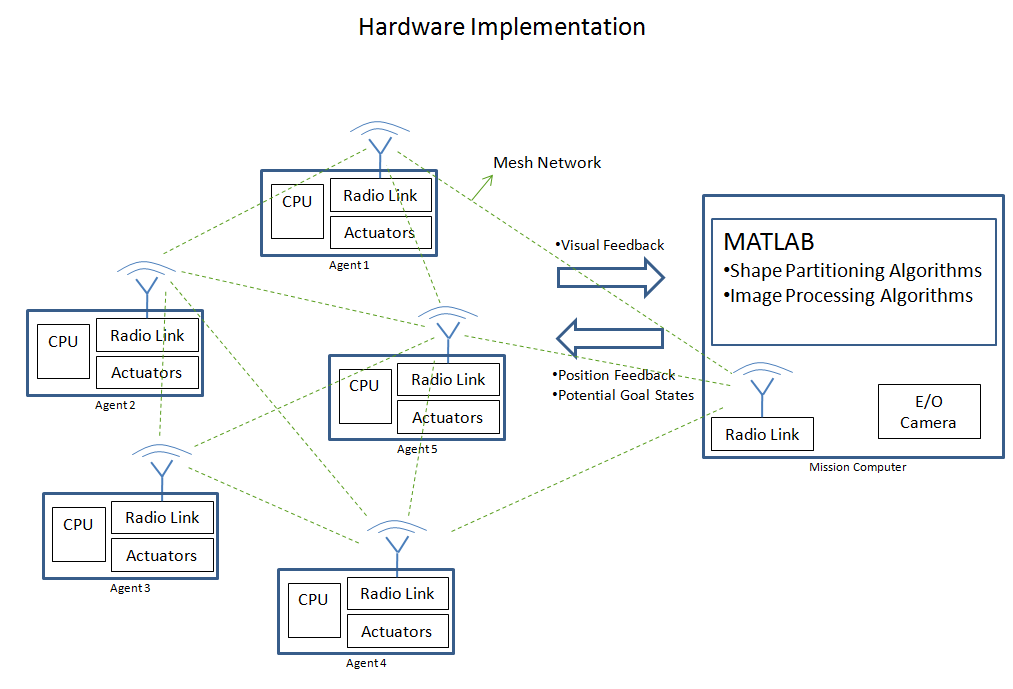
\includegraphics[scale = 0.55]{hardware}}
\end{figure} 
   
Each agent and the mission computer has a radio link to create a mesh network in which every node can transfer messages between each other directly or with the help of their neighbors. Also they can broadcast messages to the rest of the nodes in the network.  On the other hand each agent has their individual CPU to execute the goal state decision process and to control the actuators to reach the desired goal states. These processors also executes the control system which is described in Section \ref{lqr_design} and they manage the messaging operations within the mesh network.  This architecture supports the idea of partially decentralized formation control with Bubble Packing method in which each agent is responsible to take decisions and reach to a global consensus with the rest of the swarm on the potential goal states.  These potential goal states are determined by the mission computer which takes the desired formation shape from the operator and executes shape partitioning algorithms. The data of the potential goal states is broadcasted to all of the agents in the environment with the help of mesh network. 

Since the environment is an indoor area, it is impossible to use a GNSS system to provide position and velocity measurements to the agents. To provide this external measurements, a visual feedback system is used with the help of a E/O camera and image processing algorithms.  The image processing algorithms used in this work depends on the color classification of different cover planes placed on the top of the mobile robots. These covers are illustrated in Figure \ref{kapaklar_ref}

\begin{figure}[H]
\caption{Covers for Different Types of Agents} \label{kapaklar_ref}
\centerline{\includegraphics[scale = 0.10]{Kapaklar}}
\end{figure} 
		
Covers have different sizes which represents the coverage circles of the agents in 2D environment. Each cover have two different size of circles with the same color. The colors of the circles are used to classify the agent ids and the positions of the circles are used to determine both position and attitude (i.e. heading) angles of the mobile robots in the environment. The orientation of the agent in the environment is used in the command mixing algorithms of omni - wheels which will be described in details. The video of the environment is transmitted to the mission computer in nearly real time. Mission computer executes the image processing algorithms which filters the desired colors and detects the positions of the colored circles and broadcasts the position and orientation datas of the agents. A sample output of the image processing algorithm is illustrated in Figure \ref{imageprocess_ref}. 
		
\begin{figure}[H]
\caption{Sample Output of the Image Processing Algorithm} \label{imageprocess_ref}
\centerline{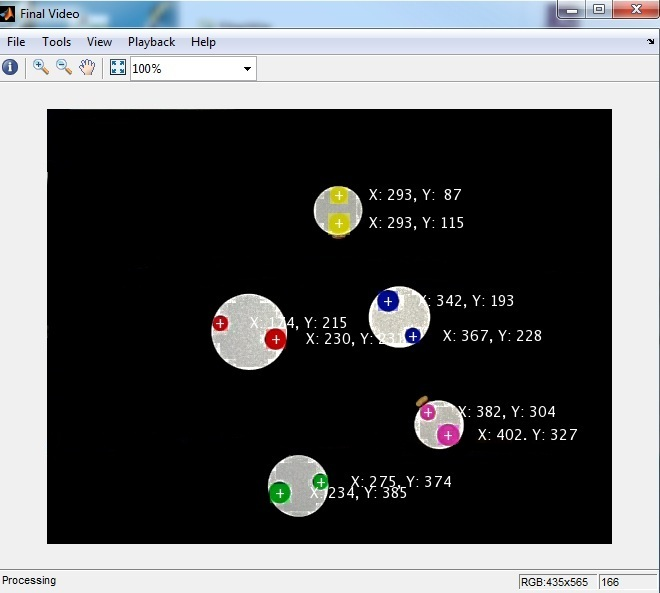
\includegraphics[scale = 0.50]{Image_Processing}}
\end{figure} 
		
The orientation of an agent is determined with the clockwise bearing angle of the vector from the center of the large circle to the center of the small circle. Figure \ref{bearing_ref} illustrates this calculation.
		
\begin{figure}[H]
\caption{Orientation of an Agent in the Environment} \label{bearing_ref}
\centerline{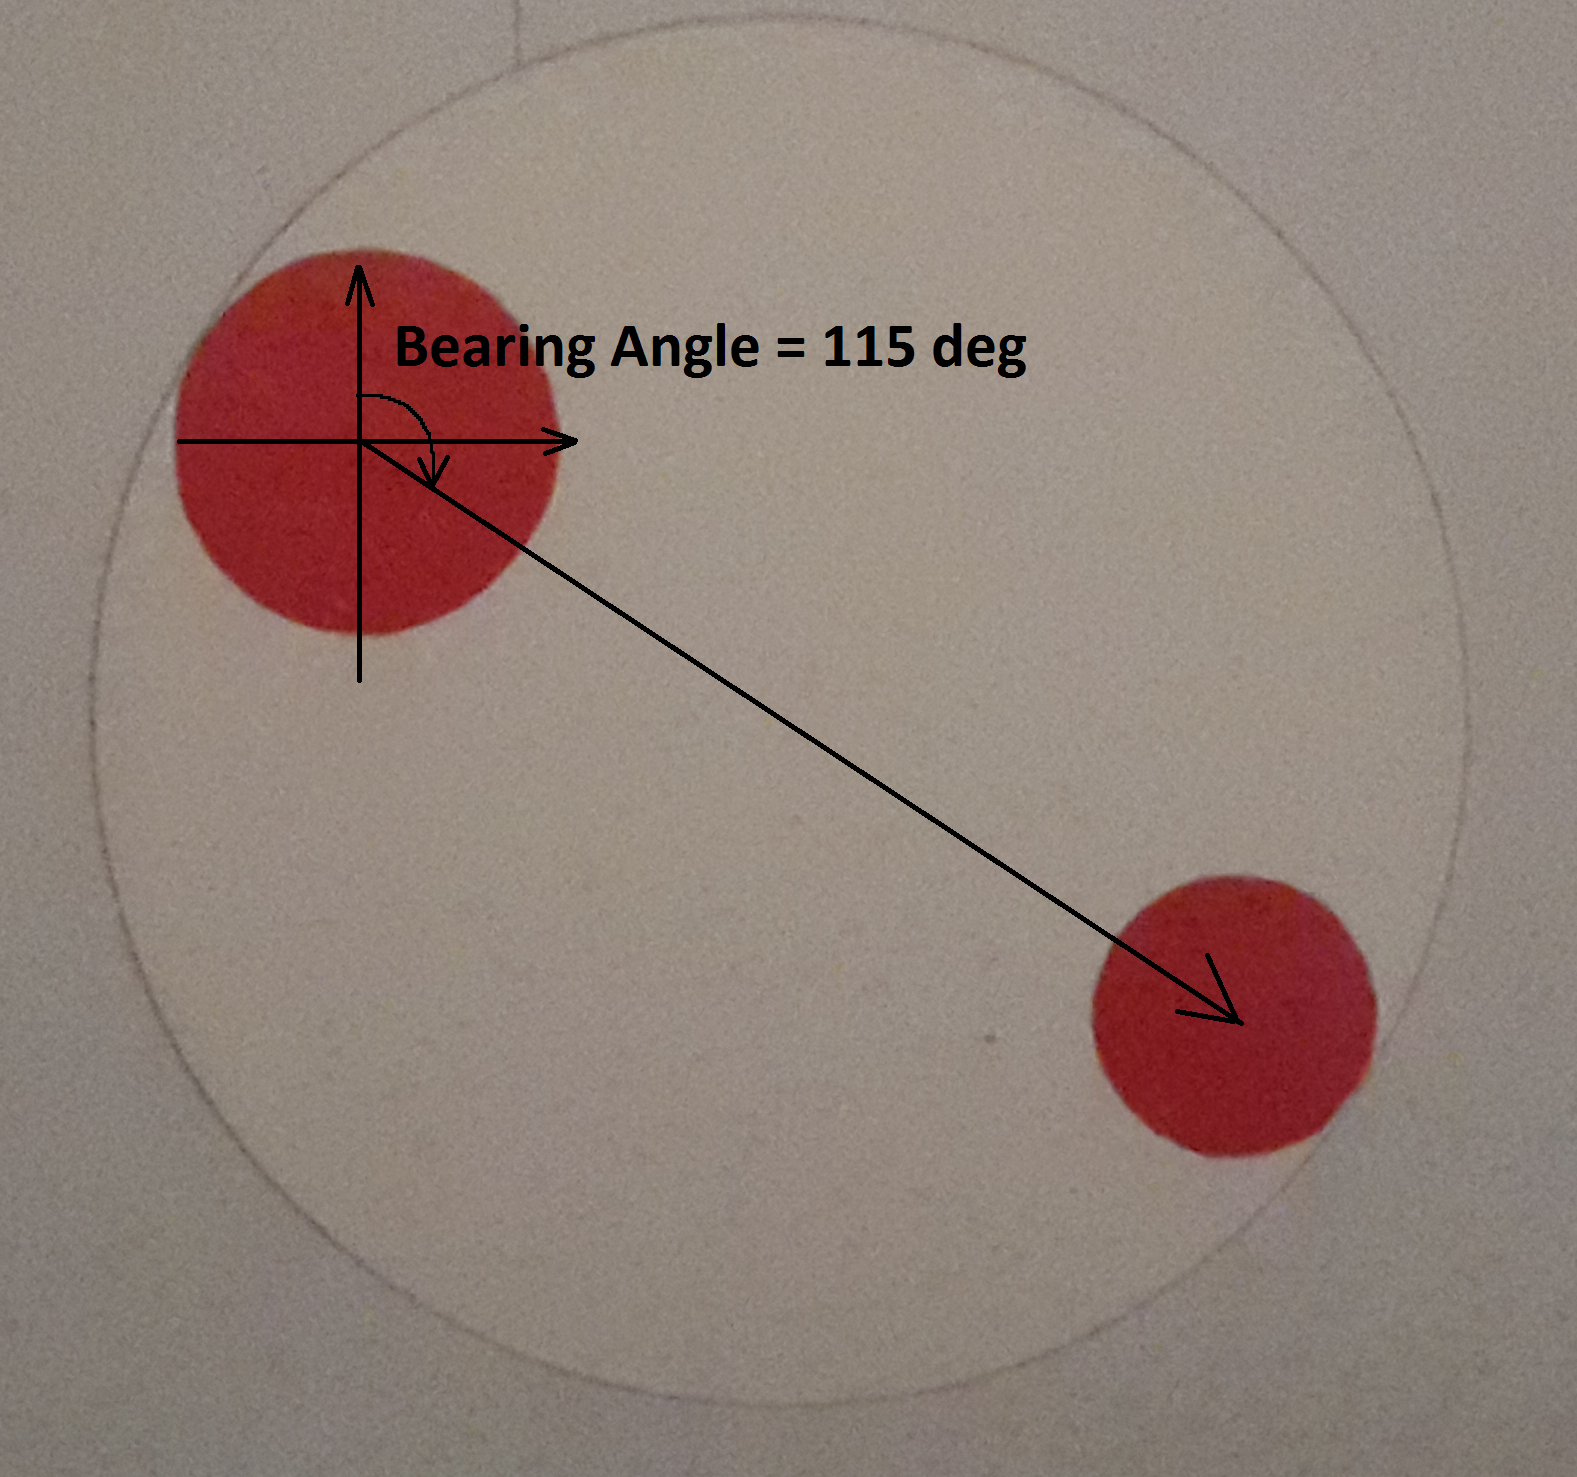
\includegraphics[scale = 0.20]{Bearing_Angle}}
\end{figure} 
		
Each agent have their individual processor unit and radio link on their boards. A block diagram of tan individual agent's harware is illustrated in Figure \ref{indhardware_ref}
		
\begin{figure}[H]
\caption{Hardware of an Agent} \label{indhardware_ref}
\centerline{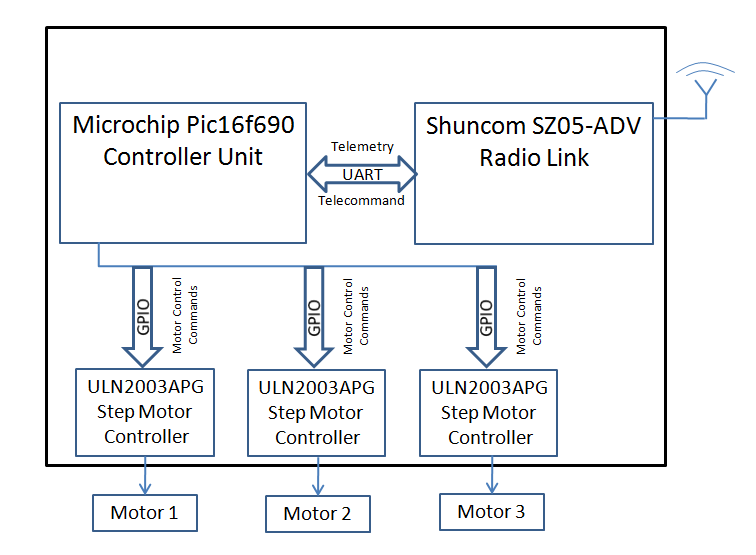
\includegraphics[scale = 0.70]{agent}}
\end{figure} 
		
Microchip's Pic16f690 Microcontroller is responsible of controlling the mobile robot and data communication with the environment. This microcontroller runs the formation control algorithms which is described in Section \ref{shapepartition_ref} and drives the 3 step motor control units, ULN2003APG, via GPIO peripherals. The instant velocity setpoints for the stepper motors  are determined with the command mixture algorithm illustrated in Figure \ref{ccmb_ref}.
		
\begin{figure}[H]
\caption{Command Mixture of Step Motors} \label{ccmb_ref}
\centerline{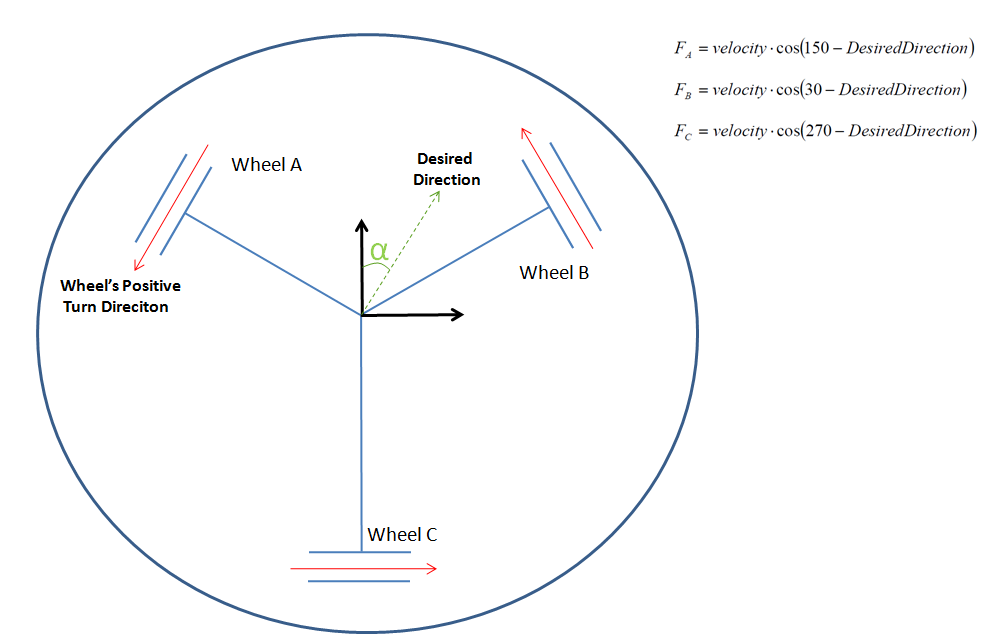
\includegraphics[scale = 0.70]{ccmb}}
\end{figure} 

The desired velocity vector for the agent is  distributed to the stepper motors in accordance with the orientation of the agent . Let $\norm{Vel}$ be the amplitude of the desired velocity and $\alpha$ is the angle representing the desired direction of the movement with respect to mobile robot's body frame.  The velocities for the stepper motors is determined with following equations,
		
\begin{align*}
& V_A = \norm{Vel} cos(150+\alpha) \\
& V_B = \norm{Vel} cos(30 +\alpha) \\
& V_C = \norm{Vel} cos(270+\alpha) 
\end{align*}  

where $V_A, V_B, V_C$ represents the desired velocities of  stepper motor A,B and C respectively.
		
Microcontroller is also drives the radio link via UART peripheral and manages the communication of the agent with the environment. All of the units on the board are supplied with a 5VDC regulator, 7805. The schematic of the circuit which controls the agent is illustrated in Figure \ref{sematik_ref} and \ref{layout_ref}.
		
\begin{figure}[H]
\caption{Schematic of the Circuit on the Board} \label{sematik_ref}
\centerline{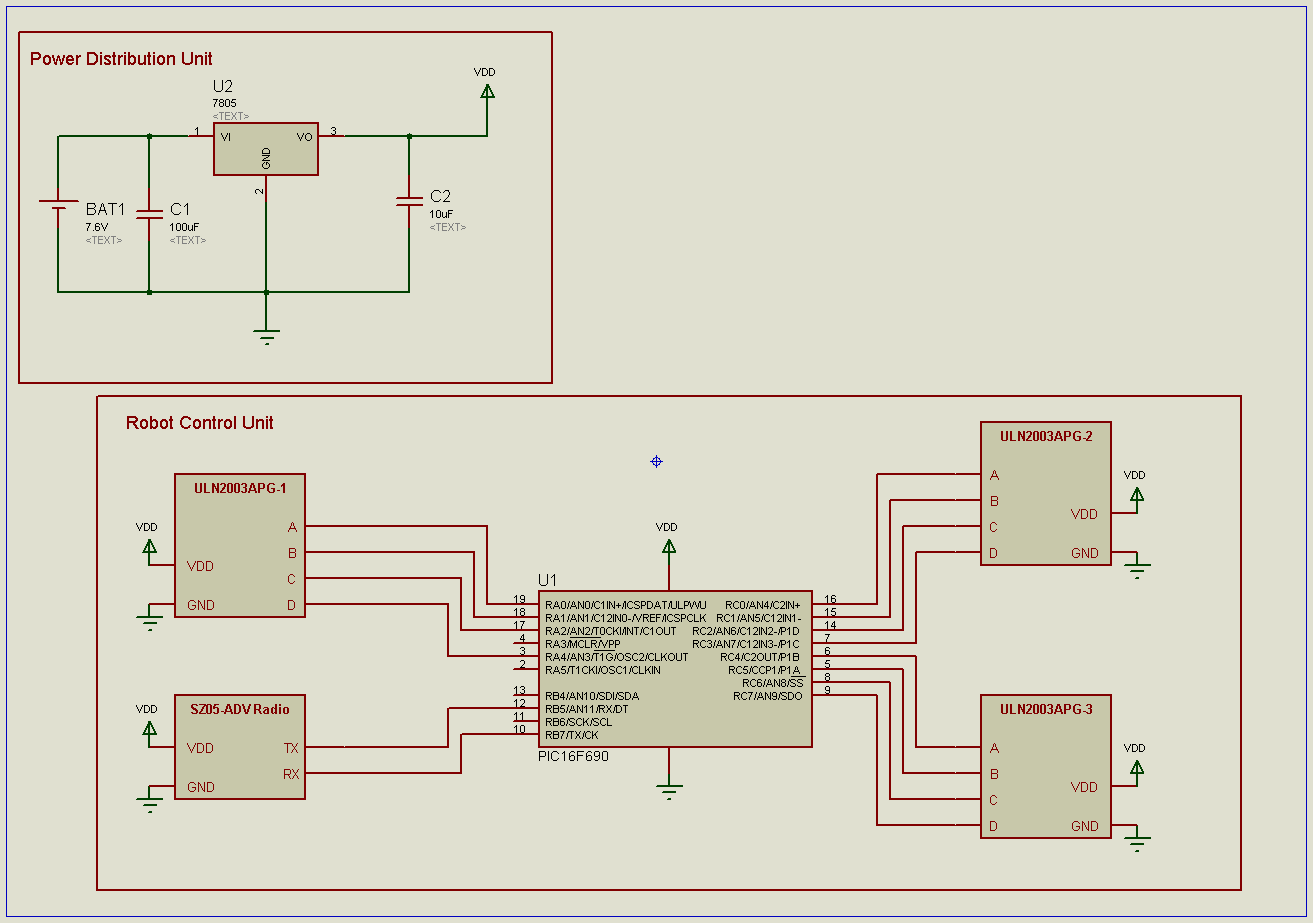
\includegraphics[scale = 0.40]{sematik}}
\end{figure} 

\begin{figure}[H]
\caption{3D Visualization of the Layout} \label{layout_ref}
\centerline{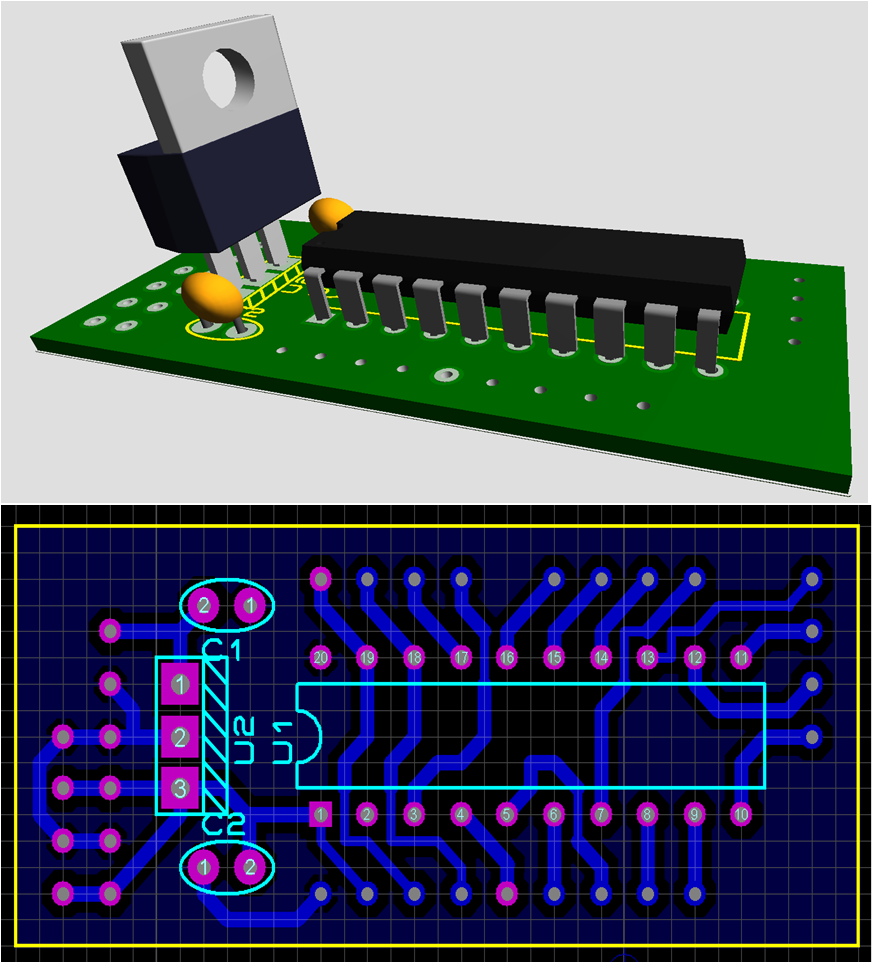
\includegraphics[scale = 0.60]{sematik-layout}}
\end{figure} 

Figure \ref{topview_ref} and Figure \ref{bottomview_ref} describes the hardware parts used on a mobile robot.

\begin{figure}[H]
\caption{Hardware of an Agent - Top View} \label{topview_ref}
\centerline{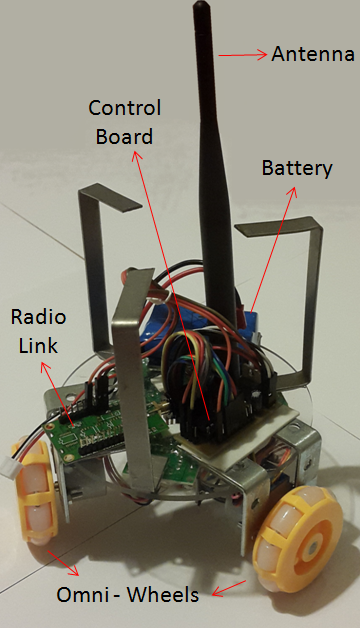
\includegraphics[scale = 0.80]{hardware1}}
\end{figure} 

\begin{figure}[H]
\caption{Hardware of an Agent - Bottom View} \label{bottomview_ref}
\centerline{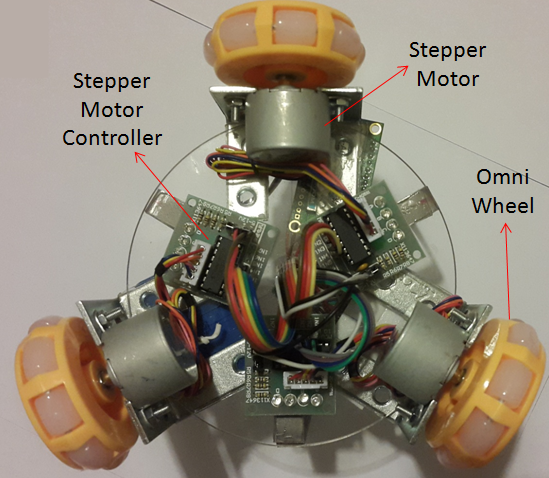
\includegraphics[scale = 0.80]{hardware2}}
\end{figure} 
		
\section{Performance Analysis}
The system is tested with several formation shapes and results are analyzed with total displacements of the agents and the settling time metrics. Sample formation shapes are covered  and the algorithm proposed for Bubble Packing method is tested in real time successfully.  Traces of the agents are plotted with the continuous blue lines from their initial positions to the goal states in the following figures. The desired formation shape is plotted with black circles. The environment is a square area which has 2x2 meter size and there are three different types of agents which have different coverage circles represented in Table \ref{agentsize_ref}

\begin{center}
\captionof{table}{Three Different Agent Configuration} \label{agentsize_ref} 
\begin{tabular}{|c| c |c |c ||}
\hline
\textbf{Agent Color}  & \textbf{Agent Type} & \textbf{Coverage Circle Radius[cm]}\\ 
\hline
Red & 1 & 16 \\
Blue & 2 & 11 \\
Green & 2 & 11 \\
Yellow & 3 & 8 \\
Pink & 3 & 8 \\
\hline
\end{tabular}
\end{center}
		
\begin{figure}[H]
\caption{Formation Shape 1- Matlab Environment}
\centerline{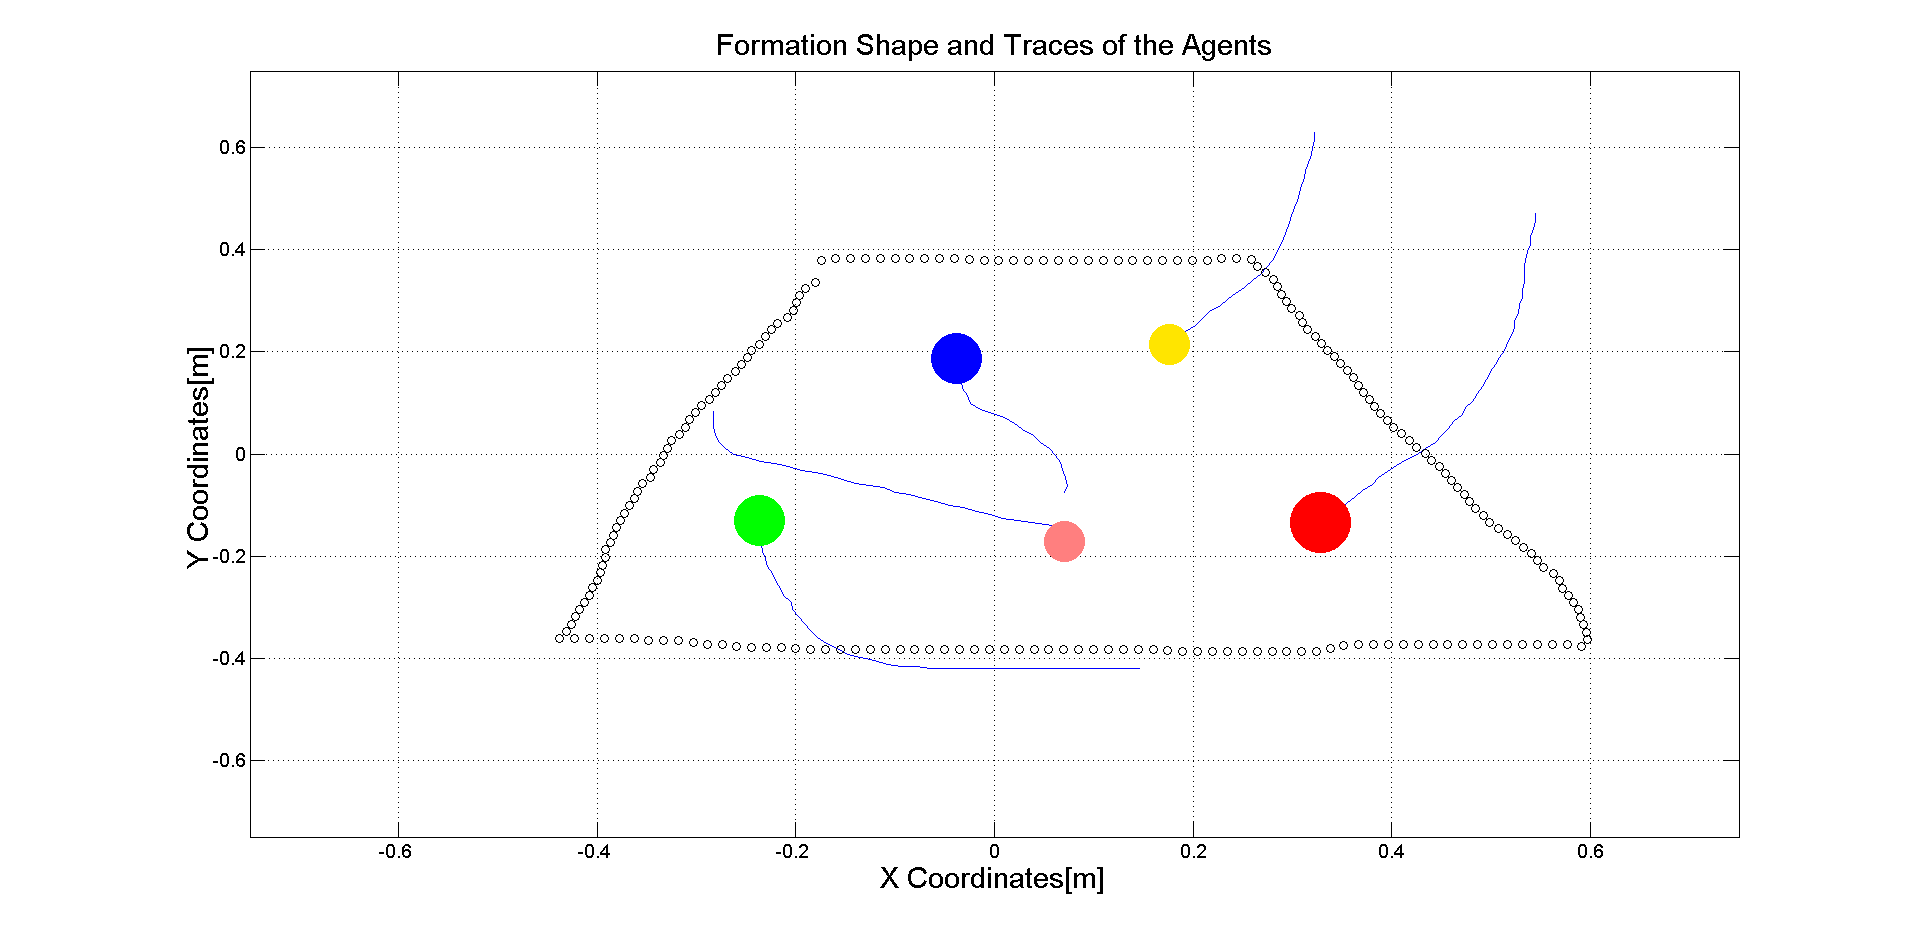
\includegraphics[scale = 0.32]{2_hardware}}
\end{figure} 
			
\begin{figure}[H]
\caption{Formation Shape 1- Test Environment}
\centerline{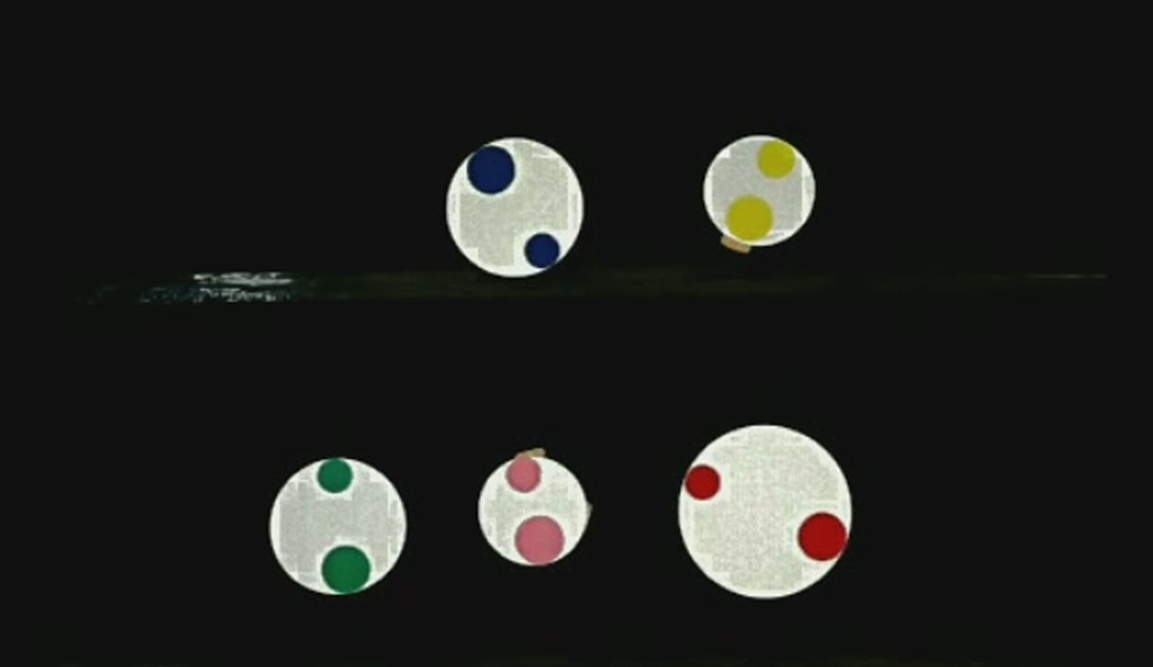
\includegraphics[scale = 0.35]{2_real_hardware}}
\end{figure} 
					
\begin{center}
\captionof{table}{Performance Metrics for Shape - 1} \label{hardwareshape1_ref} 
\begin{tabular}{||c| c |c |c ||}
\hline
\textbf{Total Displacements[m]}  & \textbf{Settling Time[sec]}\\ 
\hline
1.75 & 23 \\
\hline
\end{tabular}
\end{center}
		
\begin{figure}[H]
\caption{Formation Shape 2- Matlab Environment}
\centerline{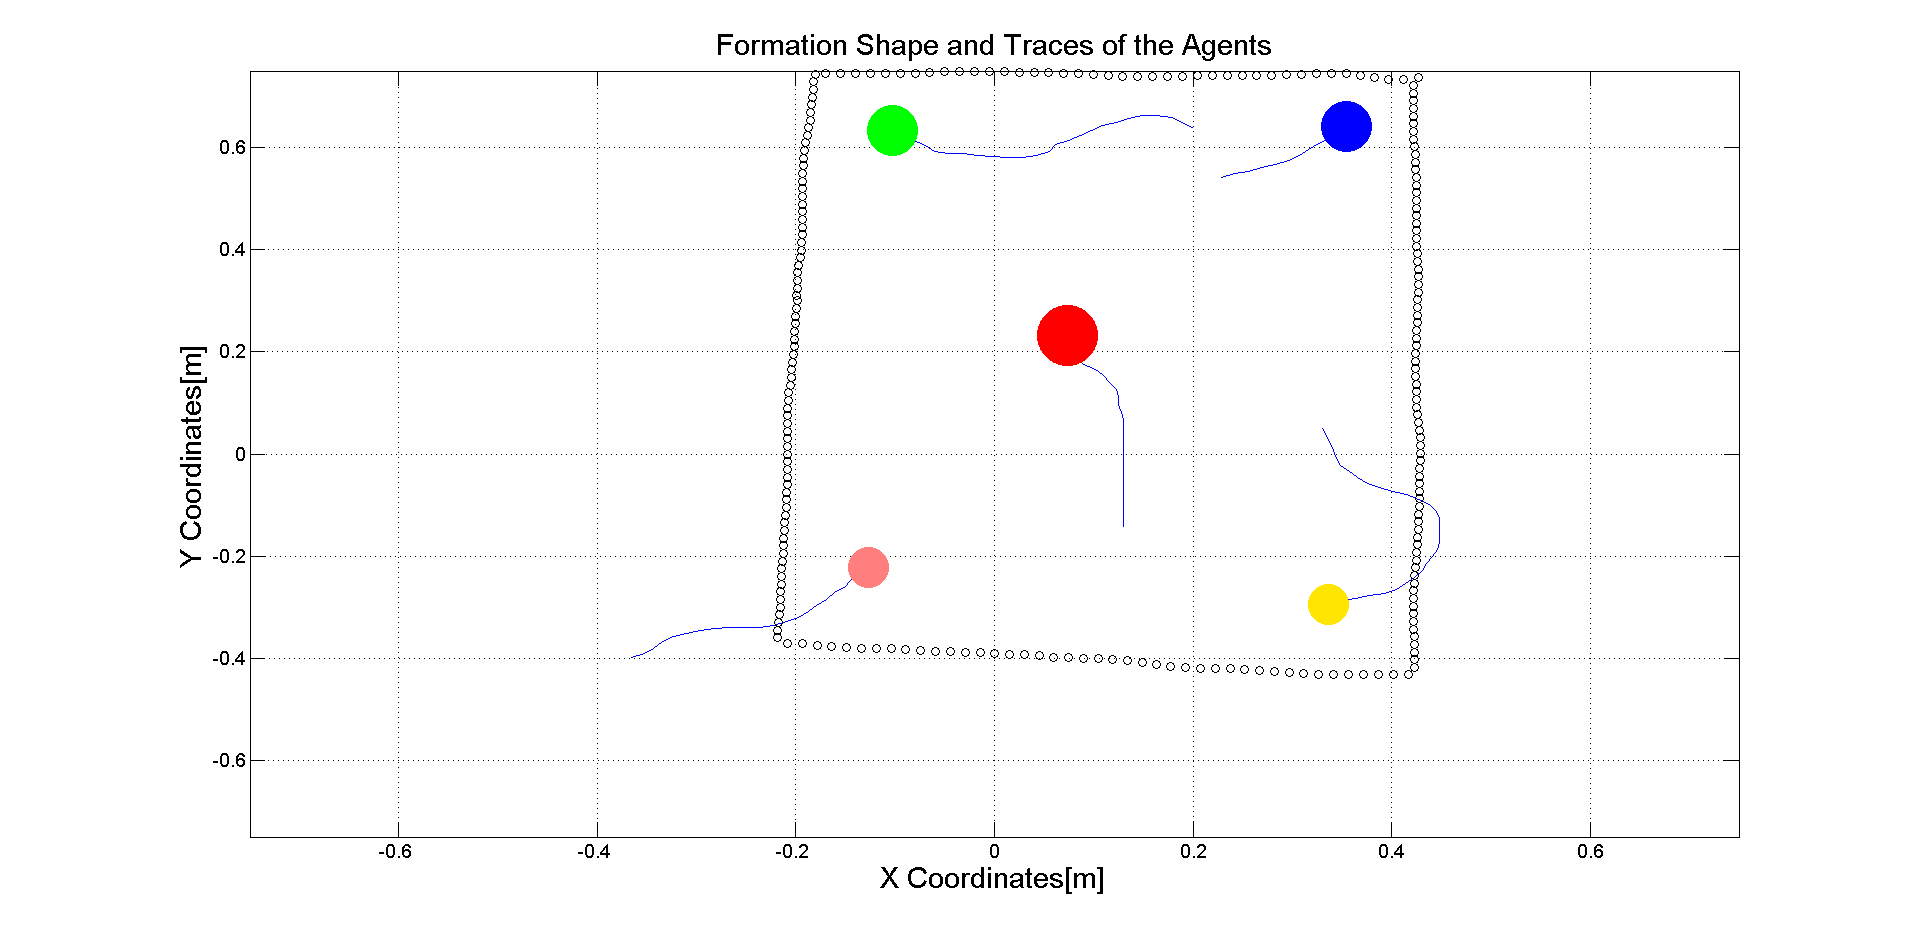
\includegraphics[scale = 0.32]{4_hardware}}
\end{figure} 
					
\begin{figure}[H]
\caption{Formation Shape 2- Test Environment}
\centerline{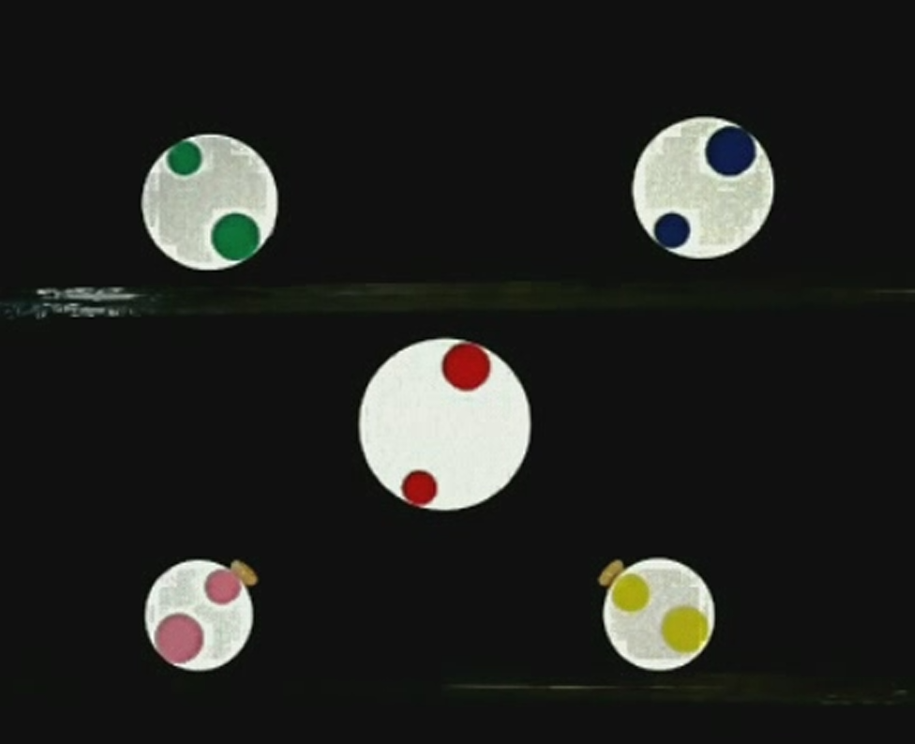
\includegraphics[scale = 0.35]{4_real_hardware}}
\end{figure} 
					
\begin{center}
\captionof{table}{Performance Metrics for Shape - 2} \label{hardwareshape2_ref} 
\begin{tabular}{||c| c |c |c ||}
\hline
\textbf{Total Displacements[m]}  & \textbf{Settling Time[sec]}\\ 
\hline
1.63 & 19 \\
\hline
\end{tabular}
\end{center}
				
\begin{figure}[H]
\caption{Formation Shape 3- Matlab Environment}
\centerline{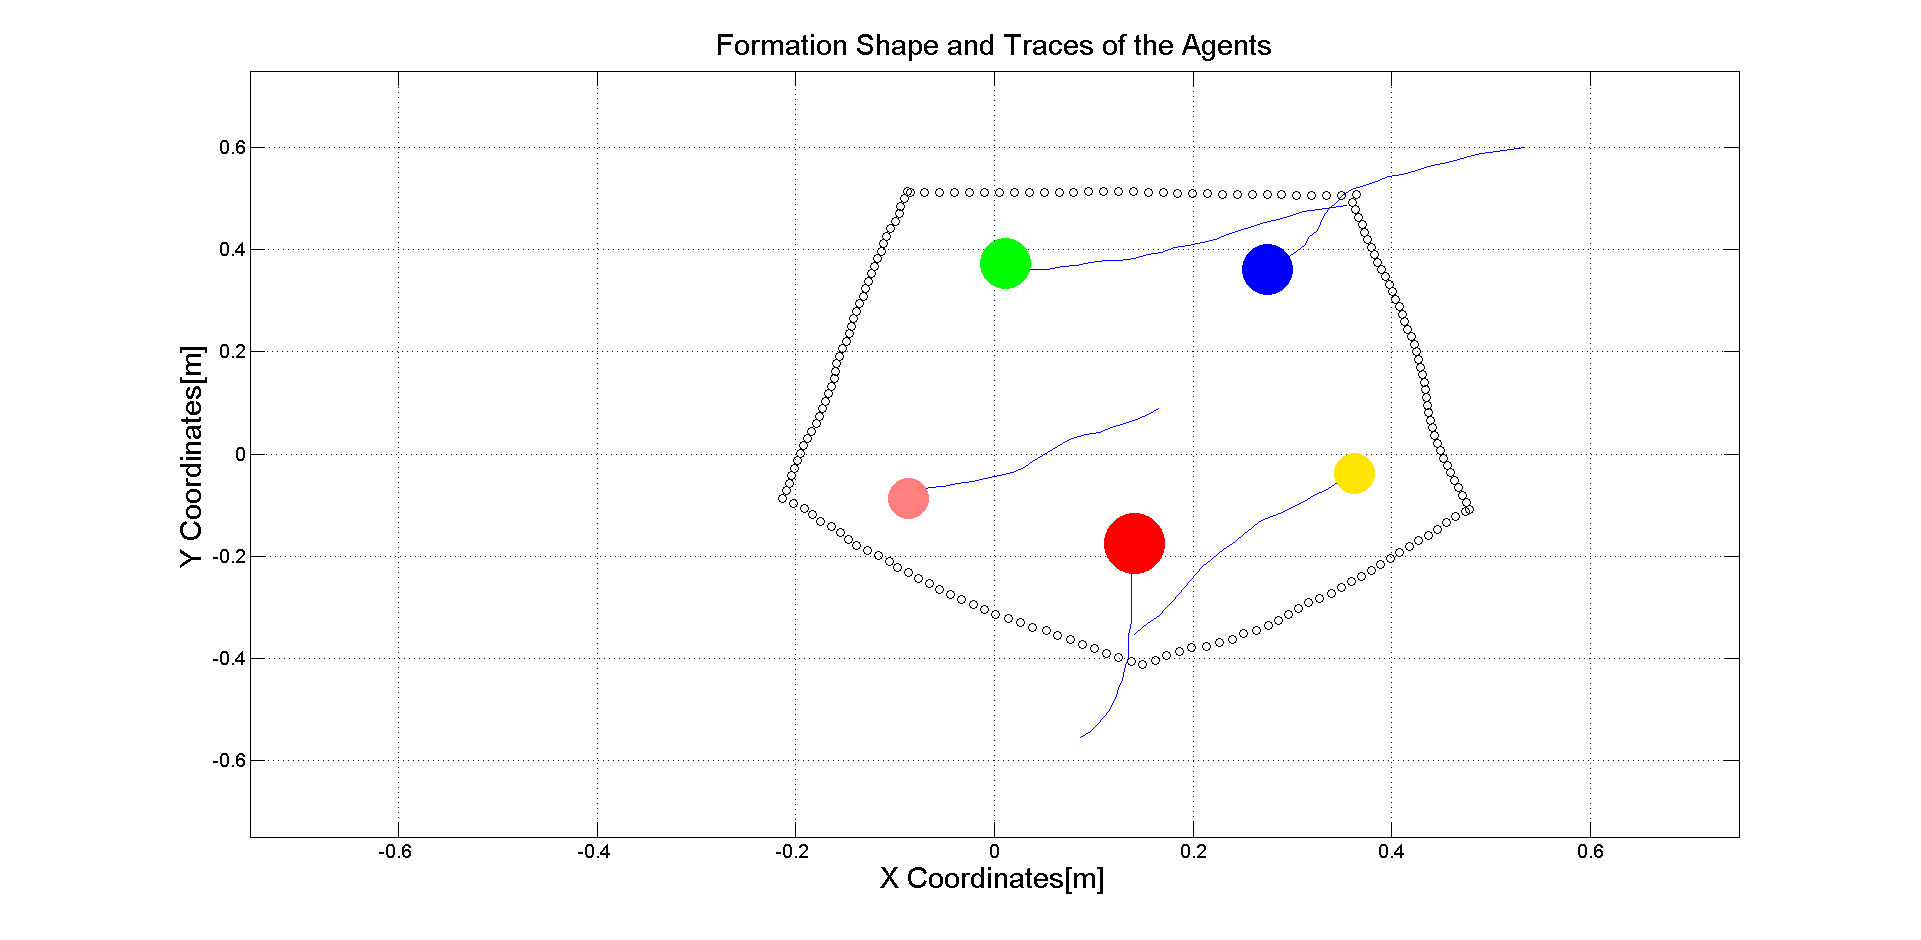
\includegraphics[scale = 0.32]{5_hardware}}
\end{figure} 
					
\begin{figure}[H]
\caption{Formation Shape 3- Test Environment}
\centerline{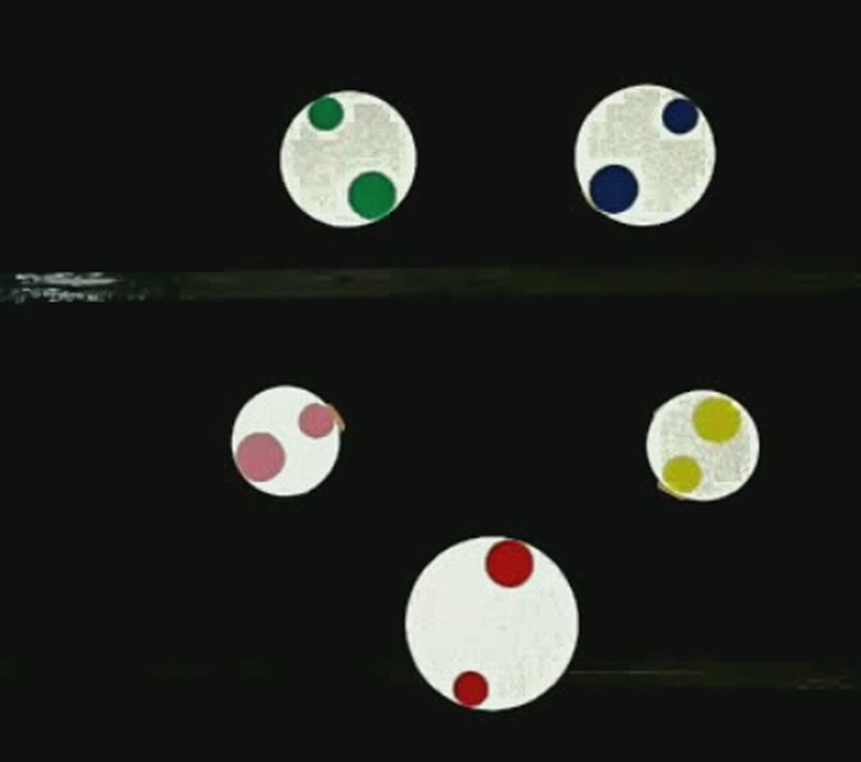
\includegraphics[scale = 0.35]{5_real_hardware}}
\end{figure} 
					
\begin{center}
\captionof{table}{Performance Metrics for Shape - 3} \label{hardwareshape3_ref} 
\begin{tabular}{||c| c |c |c ||}
\hline
\textbf{Total Displacements[m]}  & \textbf{Settling Time[sec]}\\ 
\hline
1.95 & 26 \\
\hline
\end{tabular}
\end{center}
		
\begin{figure}[H]
\caption{Formation Shape 4- Matlab Environment}
\centerline{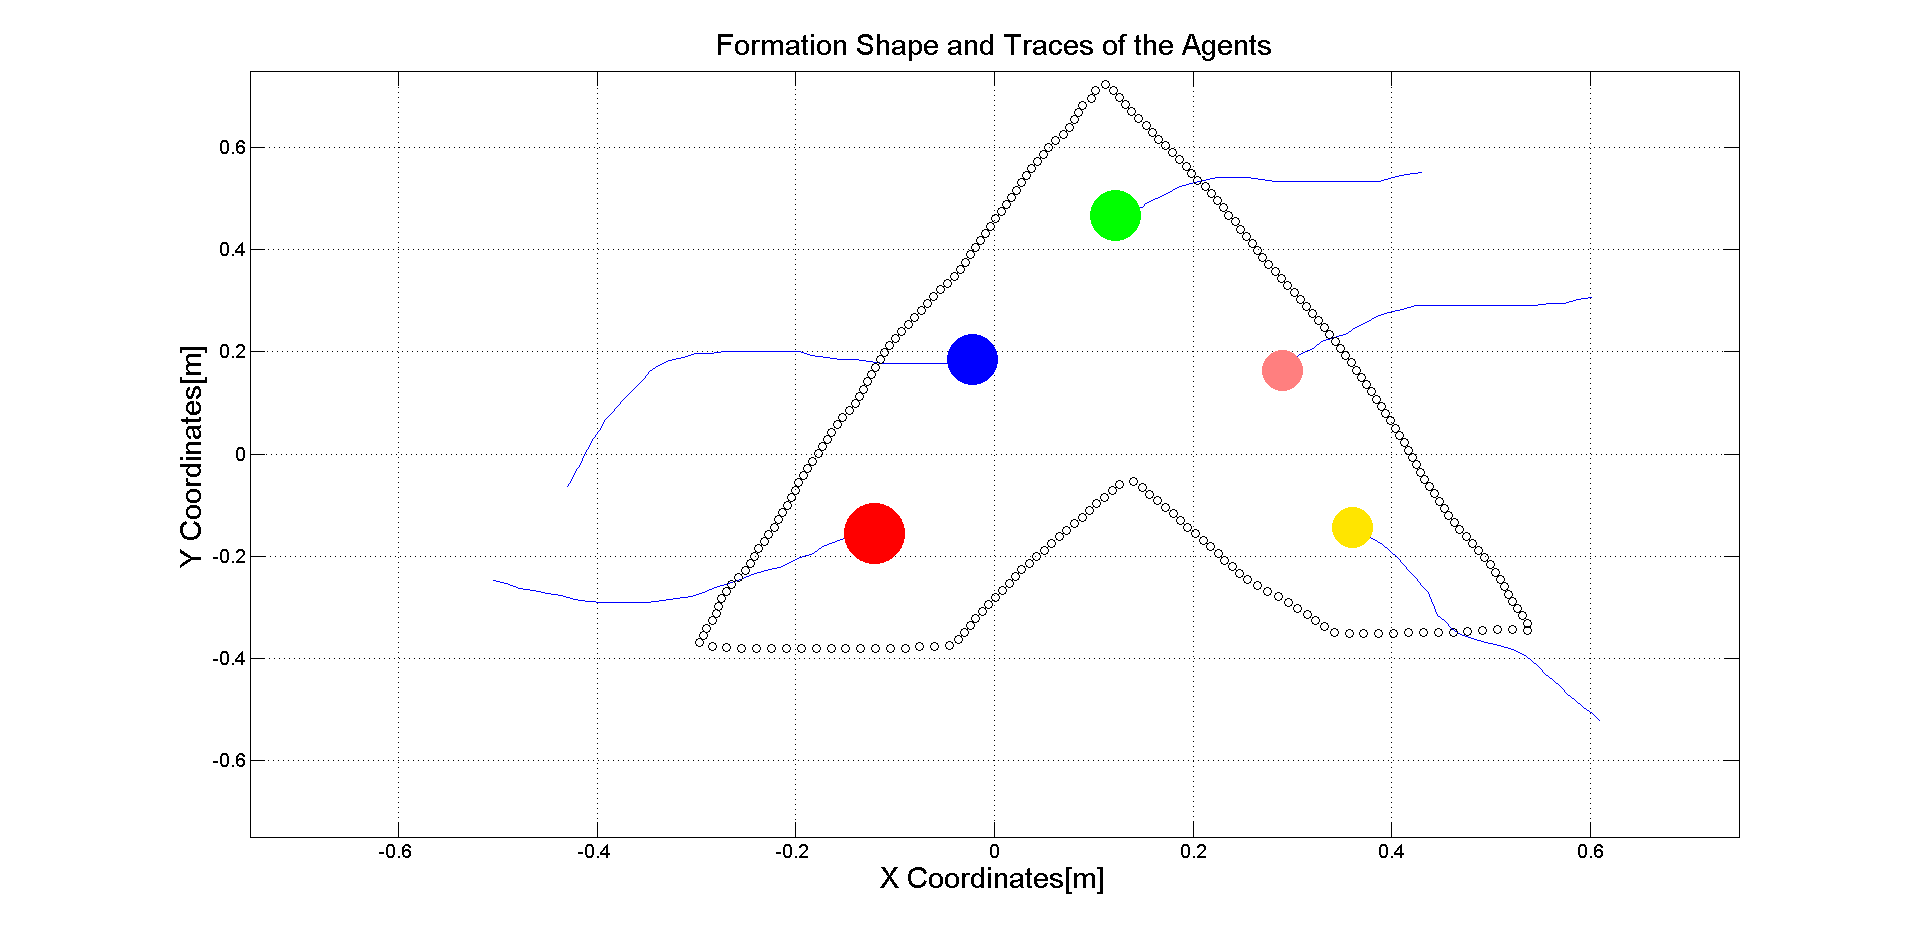
\includegraphics[scale = 0.32]{6_hardware}}
\end{figure} 
					
\begin{figure}[H]
\caption{Formation Shape 4- Test Environment}
\centerline{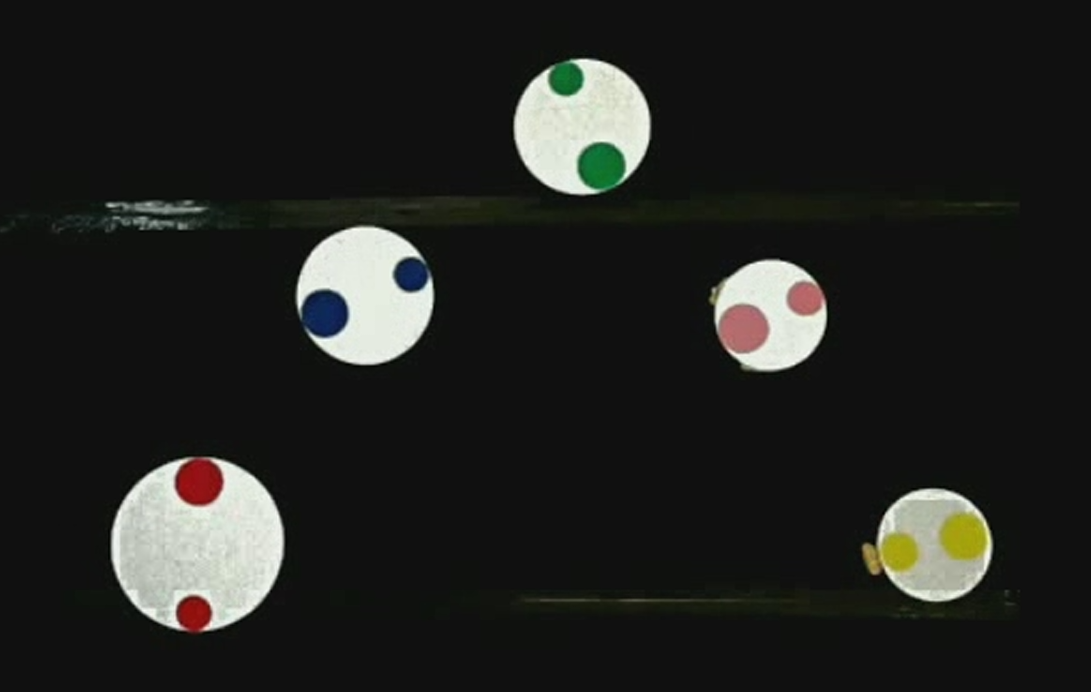
\includegraphics[scale = 0.35]{6_real_hardware}}
\end{figure} 
					
\begin{center}
\captionof{table}{Performance Metrics for Shape - 4} \label{hardwareshape4_ref} 
\begin{tabular}{||c| c |c |c ||}
\hline
\textbf{Total Displacements[m]}  & \textbf{Settling Time[sec]}\\ 
\hline
2.16 & 29 \\
\hline
\end{tabular}
\end{center}
		
\begin{figure}[H]
\caption{Formation Shape 5- Matlab Environment}
\centerline{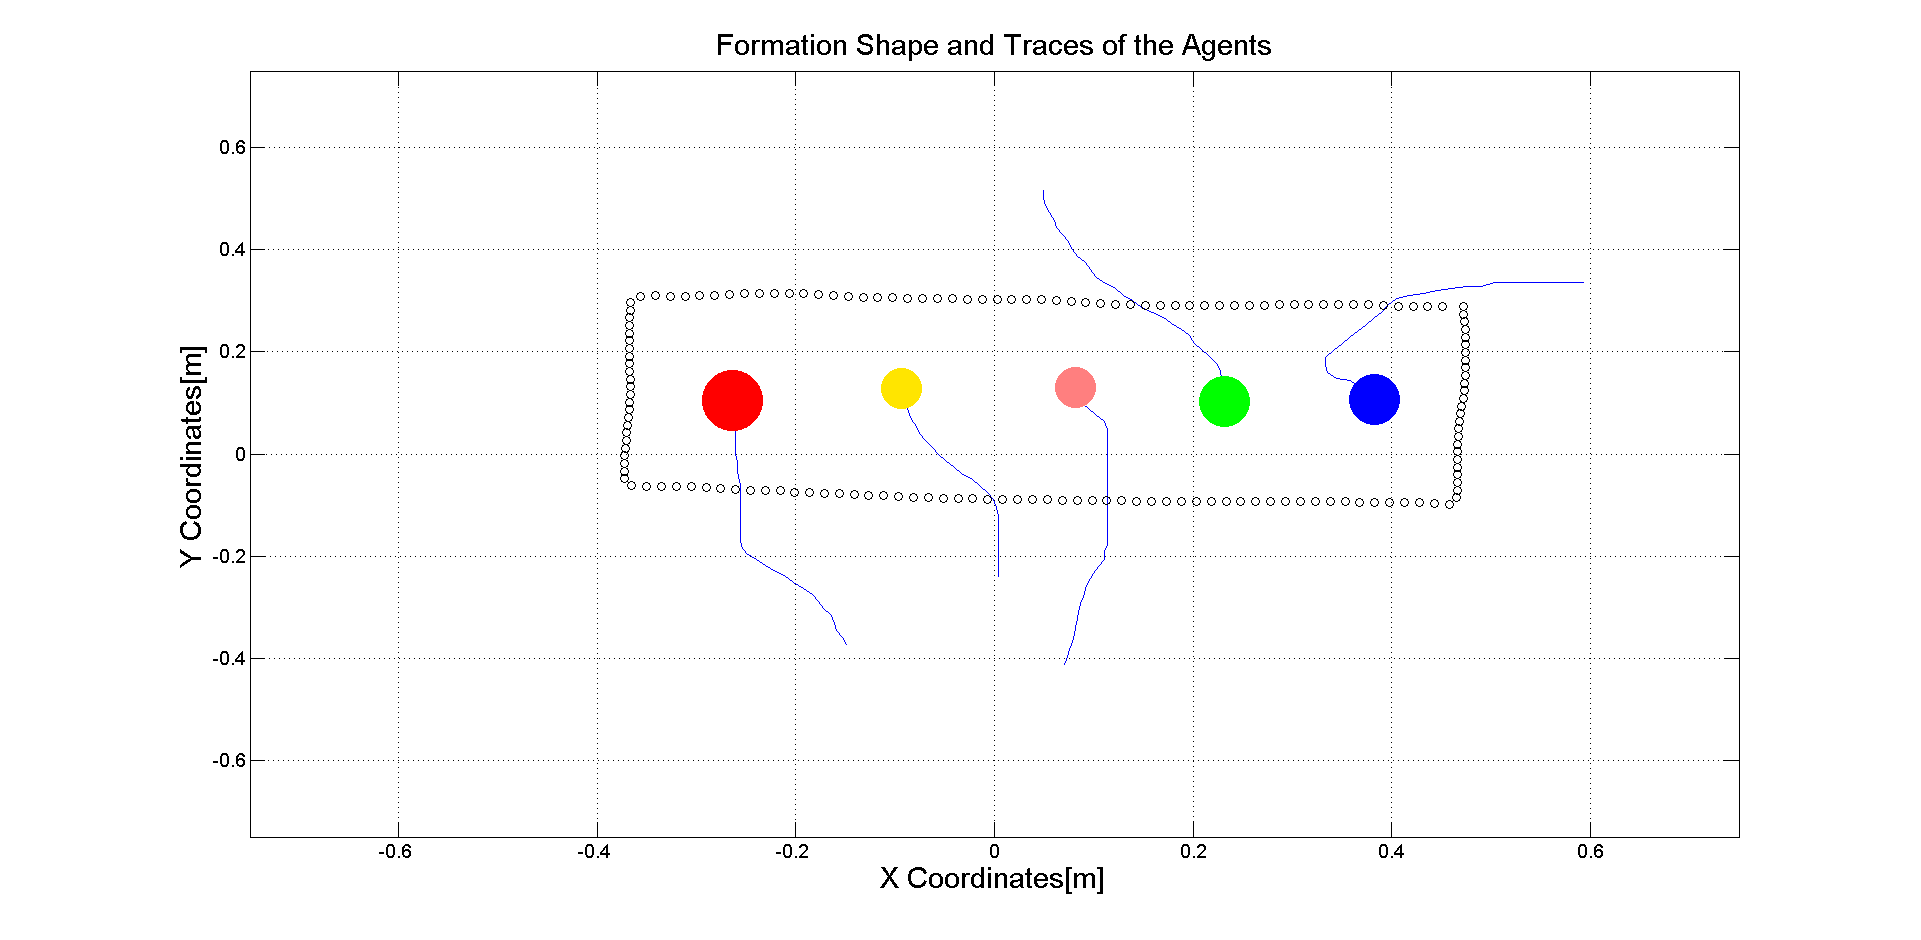
\includegraphics[scale = 0.32]{9_hardware}}
\end{figure} 
					
\begin{figure}[H]
\caption{Formation Shape 5- Test Environment}
\centerline{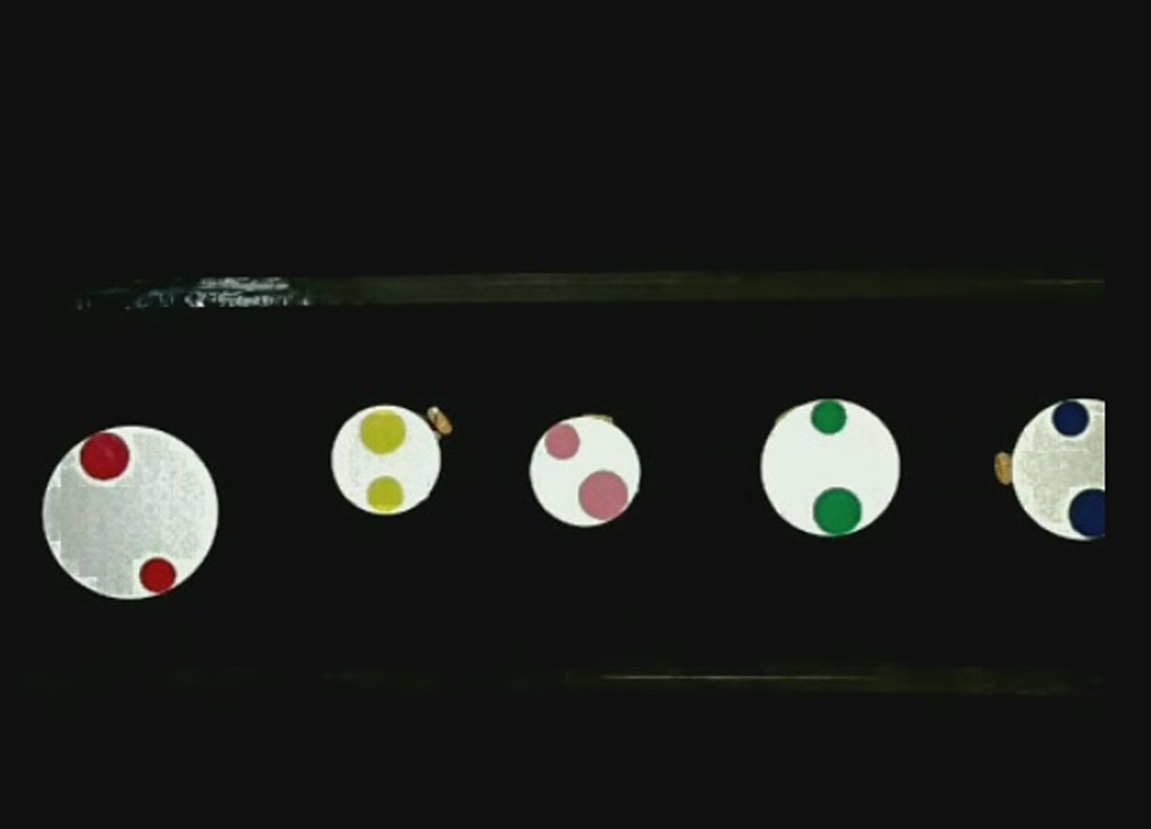
\includegraphics[scale = 0.35]{9_real_hardware}}
\end{figure} 
					
\begin{center}
\captionof{table}{Performance Metrics for Shape - 5} \label{hardwareshape5_ref} 
\begin{tabular}{||c| c |c |c ||}
\hline
\textbf{Total Displacements[m]}  & \textbf{Settling Time[sec]}\\ 
\hline
1.80 & 25 \\
\hline
\end{tabular}
\end{center}

Desired formations are simple geometrical shapes since it will not be possible to cover more complicated shaped with five agents. It is obvious that the different types of agents reaches the related goal states to minimize the total displacements. Blue and green agents (i.e. Type-2 agents) have always reached to the goal states determined for Type-2 agents by minimizing the total displacements as expected. Similarly pink and yellow agents (i.e. Type-3 agents) reached to goal states determined for Type-3 agents with total minimum displacements. 